\graphicspath{{fig/sheep/}}

\chapter{Case study I: flocking sheep}
\label{cha:sheep}

In \cref{cha:sim_studies} we showed that it is possible to infer the parameters
of a number of agent-based models from simulated data. Performing simulation
studies before attempting inference on real data is advisable as it allows an
opportunity to troubleshoot and assess the accuracy of our inference schemes.
The schemes constructed to perform inference on simulated data can now be
reused with little-to-no-alteration to perform inference on real data. With the
confidence instilled by the success of our simulation studies, if we find our
schemes unable to fit a model to \emph{real} data, we can be confident that
this is because of a discrepancy between the model and data, rather than an
error in our fitting process or our implementation of it.

This chapter shall focus on data of flocking sheep, unseen before in the
literature. Aerial footage of flocking sheep was recorded by a commercially
available drone. The position of each individual sheep was extracted from the
captured video footage using custom tracking software. In total, three flocking
sequences were extracted and analysed. The flocking events were captured and
their data extracted by Hayley Moore (thesis in preparation). Global models
considered in \cref{sec:global_models} will be fit to these sequences. The
resulting fits will be assessed for validity and ranked for performance by
Akaike Information Criteria.

\section{Flocking data}
\label{sec:data}

Aerial footage of flocking sheep was captured with a commercially available DJI
Phantom $3$ drone equipped with a built in high-definition camera, representing
a frame resolution of $4000\times3000$ pixels. This video footage was recorded
at a rate of $24$ frames per second. In total, three distinct flocking events
were captured and analysed. Each flocking event involved the same flock of $45$
sheep.

The recorded flocking events took place in large open fields: a natural
environment with which the sheep were already familiar. Flocks were recorded in
familiar terrain in an attempt to observe the most natural flocking events, and
to minimise the effect which an unfamiliar environment may have on the flock
dynamics. In some cases the flocking events were initiated by the movements of
a quad bike, but were then left to develop naturally and unprompted. Events
generally took place away from hard boundaries, such as fences and trees, but
the influence of these objects from a distance cannot be ruled-out.

Custom tracking software was constructed to determine the position of each
sheep in every video frame. To correct for the movement of the drone due to
external influences, such as wind, the resulting frames were transformed with
respect to `reference' points. Reference points are stationary and identifiable
features present in all of the captured frames. Example reference points
include field boundaries, fence posts and trees.

Having corrected for extraneous drone-movement, the captured frames were then
thresholded to separate the pixels representing sheep from their surrounding
environment. Kalman filtering and the Hungarian algorithm were then used to
track the positions of individual sheep between frames. Having linked the
positions of sheep between frames, the trajectories of motion of every
individual could be reconstructed. \cref{fig:sheep_frame} shows the positions
of sheep in a single video frame, overlain are the positions of these sheep in
previous frames.

\begin{figure}[tbp]
  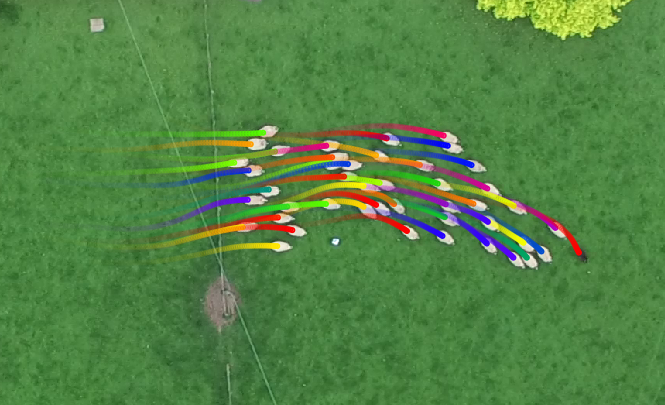
\includegraphics[width=0.8\textwidth]{traj0130_crop.png}
  \caption{A visualisation of data realised from a single flocking event. The
    faint vertical line seen passing through the image shows a boundary fence
    which was located here previously. The position of each sheep in every
    video frame was extracted using custom tracking software. Coloured lines
    represent the positions of sheep in previous frames. Each flocking event
    tracked the movements of $45$ sheep over $\approx200$ frames. A single
    flocking sequence then represents approximately $45\times200=9,000$
    observations. Footage was recorded at a rate of 24 frames per second, and so
    each sequence represents $\approx10$\,seconds of raw footage.}
  \label{fig:sheep_frame}
\end{figure}

Having realised the trajectories of each individual it is then a simple process
to determine the velocity, speed and direction of motion of each individual.
Using \cref{eq:alignment} it is possible to compute the mean polarisation of
the flocks in each sequence. The attributes of each flocking event are
summarised in \cref{tab:data_summary}. We see that sequences are broadly
similar: representing highly-polarised flocks moving at similar speeds.

\begin{table}[tbp]
\begin{tabular}{@{}crrrr@{}}
\toprule
Sequence & Frames & Sheep & Mean speed (px\,s$^{-1}$) & Mean alignment \\
\midrule
1 &    192 &     45 &      4.20 &          0.99 \\
2 &    183 &     45 &      3.26 &          0.98 \\
3 &    194 &     45 &      4.25 &          0.97 \\
\bottomrule
\end{tabular}
\caption{Summaries of the three flocking sequences analysed in this chapter.
  Each sequence involved a flock of the same $45$ sheep, recorded over
  $\approx200$ frames. As the data was recorded at a rate of $24$ frames per
  second, each sequence represents around $10$ seconds of raw footage. The
  observed flocks were all highly polarized and moved at similar speeds.}
\label{tab:data_summary}
\end{table}

\cref{fig:seq_1_traj,fig:seq_2_traj,fig:seq_3_traj} show the trajectories of
motion of each individual in the three recorded flocking events. The positions
of sheep in the first frame of the video are represented by red markers. The
sheep then travel along the blue lines, with their last recorded position
illustrated by the green markers.

\begin{figure}[tbp]
  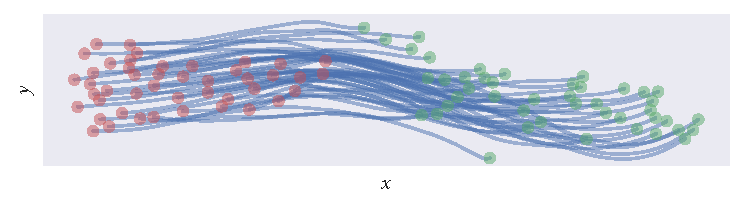
\includegraphics{seq_1_traj.pdf}
  \caption{The trajectories of sheep reconstructed from video footage of
  sequence one. The realised flock shows $45$ individuals moving cohesively
  over $192$ frames. The observations in the first frame of this sequence were
  used to seed the forward simulations in \cref{cha:sim_studies}.}
  \label{fig:seq_1_traj}
\end{figure}
\begin{figure}[tbp]
  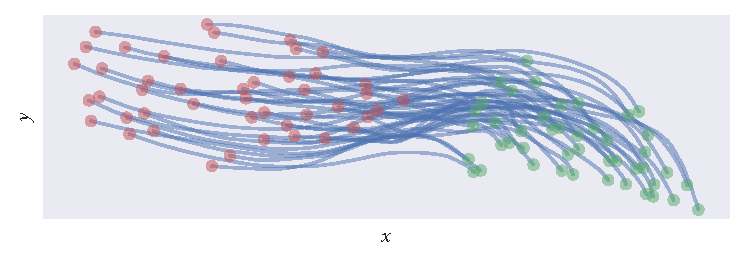
\includegraphics{seq_2_traj.pdf}
  \caption{The movement of sheep in the second sequence recorded. These
  trajectories correspond to those shown in the drone footage of
  \cref{fig:sheep_frame}.}
  \label{fig:seq_2_traj}
\end{figure}
\begin{figure}[tbp]
  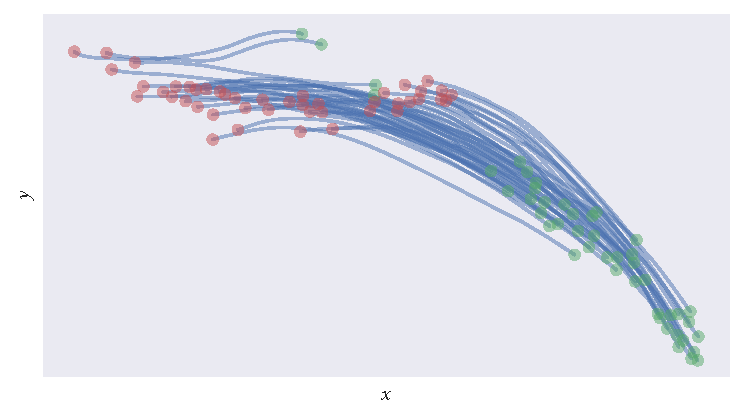
\includegraphics{seq_3_traj.pdf}
  \caption{An illustration of the movements in recorded sequence three. This
  flock goes through larger changes in direction than seen in sequences
  one and two, but remains just as cohesive.}
  \label{fig:seq_3_traj}
\end{figure}

The data realised by the drone captured footage resembles the data used in the
simulation studies of \cref{cha:sim_studies}. In fact, the first observed frame
of sequence 1 was used to seed these forward simulations.
    
\section{Model fitting}

We shall now proceed to fit the global agent-based models introduced in
\cref{cha:model_dev} to our three realised sequences. The performance of these
fitted models will be assess by the Akaike Information Criteria. Model adequacy
will be inspected with residual plots.

\subsection{Sequence 1}

Sequence 1 represents the most cohesive flocking event of those captured. We
shall begin by fitting the Null, Vicsek, power-law weighted, Gaussian weighted
and topological models to the data. Having completed the fitting, we may then
assess their adequacy by inspecting plots of the resulting standardised
residuals. To compare the performance of the models considered we use the
Akaike Information Criteria, and Akaike weights.

\subsubsection{Posterior beliefs}

% vspace filth
% a proper solution would be modify the lengths \abovecaptionskip
% and \belowcaptionskip

\begin{figure}[p]
  \captionsetup[subfigure]{aboveskip=0pt,
                           belowskip=9pt,
                           oneside,
                           margin={0.7cm,0cm}}
  \begin{subfigure}[b]{\textwidth}
    \centering
    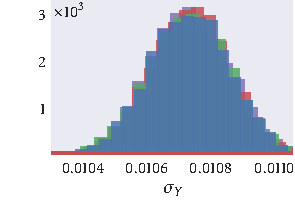
\includegraphics{seq1/null_hist_sigma_Y.pdf}%
    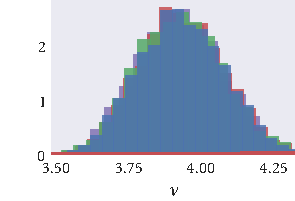
\includegraphics{seq1/null_hist_nu.pdf}
    \caption{Null model}
  \end{subfigure}
  \begin{subfigure}[b]{\textwidth}
    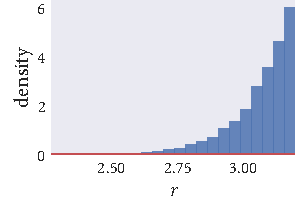
\includegraphics{seq1/r_hist_r.pdf}%
    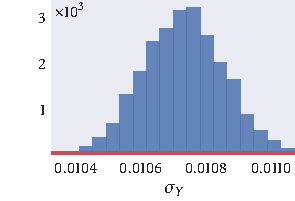
\includegraphics{seq1/r_hist_sigma_Y.pdf}%
    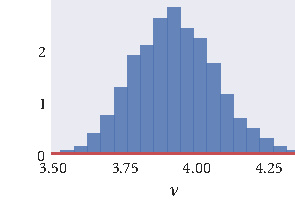
\includegraphics{seq1/r_hist_nu.pdf}
    \caption{Vicsek model}
  \end{subfigure}
  \begin{subfigure}[b]{\textwidth}
    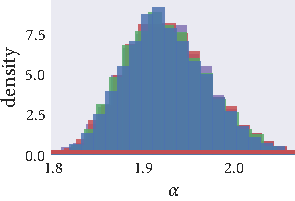
\includegraphics{seq1/power_hist_alpha.pdf}%
    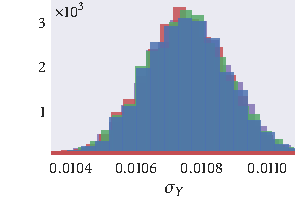
\includegraphics{seq1/power_hist_sigma_Y.pdf}%
    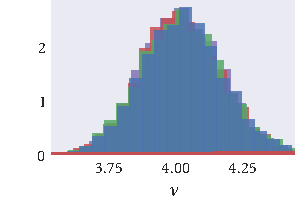
\includegraphics{seq1/power_hist_nu.pdf}
    \caption{Power-law weighted model}
  \end{subfigure}
  \begin{subfigure}[b]{\textwidth}
    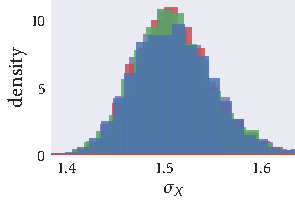
\includegraphics{seq1/gauss_hist_sigma_X.pdf}%
    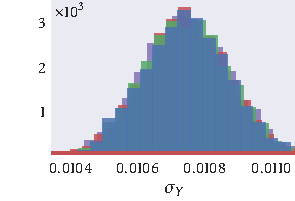
\includegraphics{seq1/gauss_hist_sigma_Y.pdf}%
    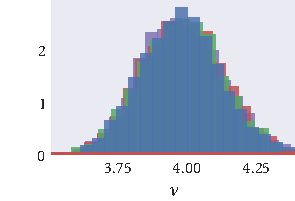
\includegraphics{seq1/gauss_hist_nu.pdf}
    \caption{Gaussian weighted model}
  \end{subfigure}
  \begin{subfigure}[b]{\textwidth}
    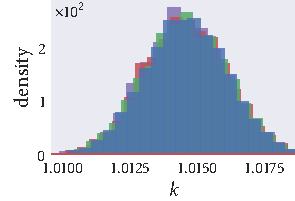
\includegraphics{seq1/top_hist_k.pdf}%
    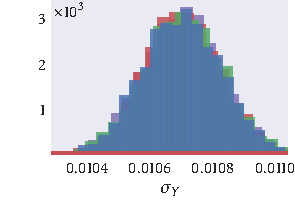
\includegraphics{seq1/top_hist_sigma_Y.pdf}%
    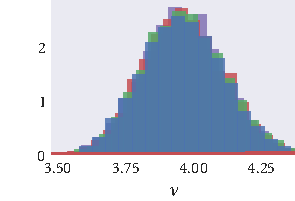
\includegraphics{seq1/top_hist_nu.pdf}%
    \caption{Topological model}
  \end{subfigure}
  \caption{Posterior beliefs of model fits to sequence $1$.}
\end{figure}

\subsubsection{Standardised residuals}

\begin{figure}
  \captionsetup[subfigure]{aboveskip=2pt,
                           belowskip=9pt,
                           oneside,
                           margin={0.7cm,0cm}}
  \begin{subfigure}[b]{0.33333\textwidth}
    \caption{Null model}
    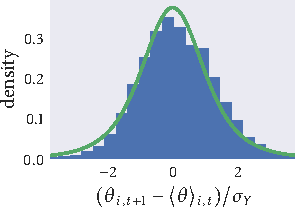
\includegraphics{seq1/null_residuals.pdf}
  \end{subfigure}\hspace{2pt}
  \begin{subfigure}[b]{0.33333\textwidth}
    \caption{Vicsek model}
    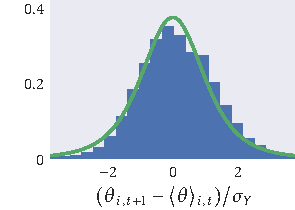
\includegraphics{seq1/r_residuals.pdf}
  \end{subfigure}\vspace{1em}\\
  \begin{subfigure}[b]{0.33333\textwidth}
    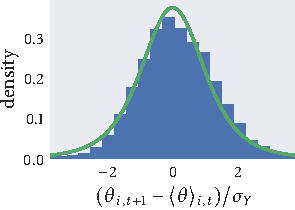
\includegraphics{seq1/power_residuals.pdf}
    \caption{Power-law weighted model}
  \end{subfigure}%
  \begin{subfigure}[b]{0.33333\textwidth}
    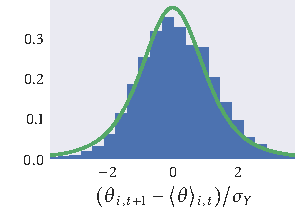
\includegraphics{seq1/gauss_residuals.pdf}
    \caption{Gaussian weighted model}
  \end{subfigure}%
  \begin{subfigure}[b]{0.33333\textwidth}
    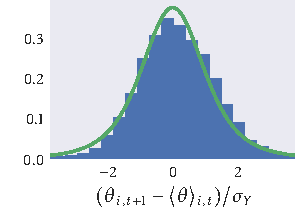
\includegraphics{seq1/top_residuals.pdf}
    \caption{Topological model}
  \end{subfigure}
  \caption{Standardised residuals of models fitted to sequence $1$.}
\end{figure}

\subsubsection{Model rankings}

\subsubsection{Posterior predictive checks}

\subsection{Sequence 2}

\subsubsection{Posterior beliefs}

\begin{figure}[p]
  \captionsetup[subfigure]{aboveskip=0pt,
                           belowskip=9pt,
                           oneside,
                           margin={0.7cm,0cm}}
  \begin{subfigure}[b]{\textwidth}
    \centering
    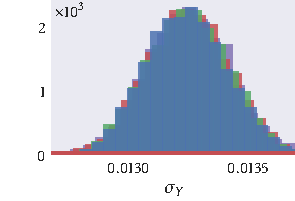
\includegraphics{seq2/null_hist_sigma_Y.pdf}\hspace{0.01\textwidth}
    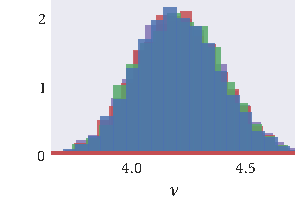
\includegraphics{seq2/null_hist_nu.pdf}
    \caption{Null model}
  \end{subfigure}
  \begin{subfigure}[b]{\textwidth}
    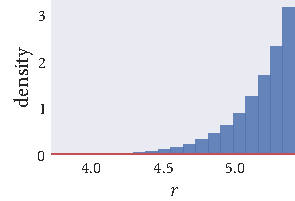
\includegraphics{seq2/r_hist_r.pdf}%
    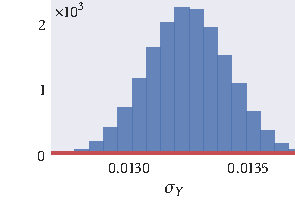
\includegraphics{seq2/r_hist_sigma_Y.pdf}%
    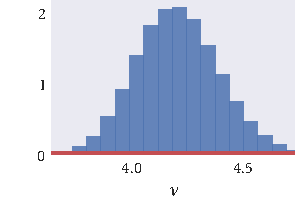
\includegraphics{seq2/r_hist_nu.pdf}
    \caption{Vicsek model}
  \end{subfigure}
  \begin{subfigure}[b]{\textwidth}
    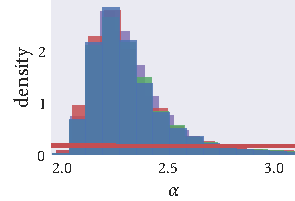
\includegraphics{seq2/power_hist_alpha.pdf}%
    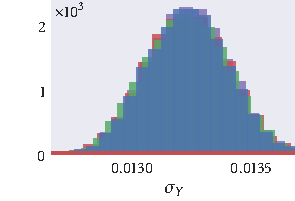
\includegraphics{seq2/power_hist_sigma_Y.pdf}%
    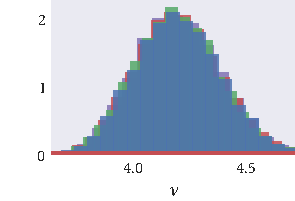
\includegraphics{seq2/power_hist_nu.pdf}
    \caption{Power-law weighted model}
  \end{subfigure}
  \begin{subfigure}[b]{\textwidth}
    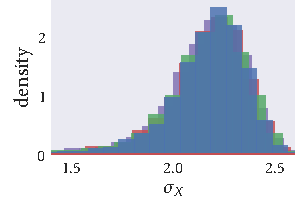
\includegraphics{seq2/gauss_hist_sigma_X.pdf}%
    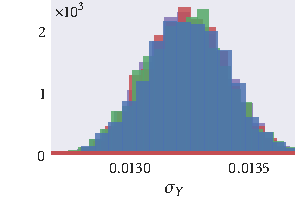
\includegraphics{seq2/gauss_hist_sigma_Y.pdf}%
    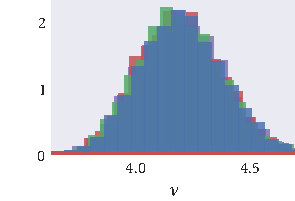
\includegraphics{seq2/gauss_hist_nu.pdf}
    \caption{Gaussian weighted model}
  \end{subfigure}
  \begin{subfigure}[b]{\textwidth}
    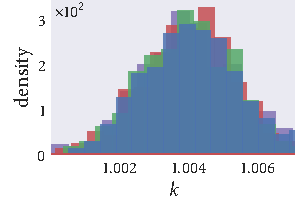
\includegraphics{seq2/top_hist_k.pdf}%
    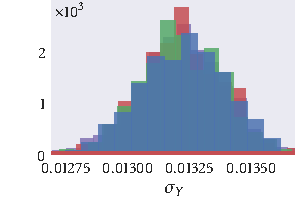
\includegraphics{seq2/top_hist_sigma_Y.pdf}%
    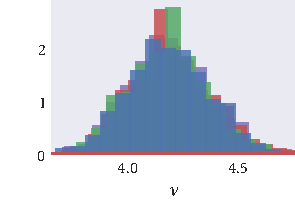
\includegraphics{seq2/top_hist_nu.pdf}%
    \caption{Topological model}
  \end{subfigure}
  \caption{Posterior beliefs of model fits to sequence $2$.}
\end{figure}

\subsubsection{Standardised residuals}

\begin{figure}
  \captionsetup[subfigure]{aboveskip=2pt,
                           belowskip=9pt,
                           oneside,
                           margin={0.7cm,0cm}}
  \begin{subfigure}[b]{0.33333\textwidth}
    \caption{Null model}
    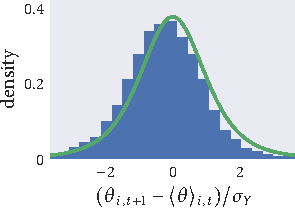
\includegraphics{seq2/null_residuals.pdf}
  \end{subfigure}\hspace{2pt}
  \begin{subfigure}[b]{0.33333\textwidth}
    \caption{Vicsek model}
    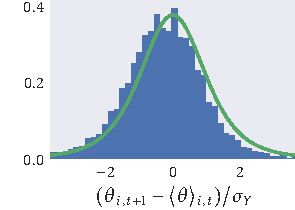
\includegraphics{seq2/r_residuals.pdf}
  \end{subfigure}\vspace{1em}\\
  \begin{subfigure}[b]{0.33333\textwidth}
    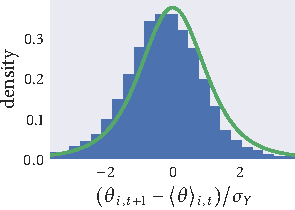
\includegraphics{seq2/power_residuals.pdf}
    \caption{Power-law weighted model}
  \end{subfigure}%
  \begin{subfigure}[b]{0.33333\textwidth}
    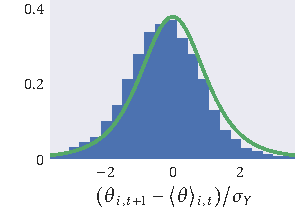
\includegraphics{seq2/gauss_residuals.pdf}
    \caption{Gaussian weighted model}
  \end{subfigure}%
  \begin{subfigure}[b]{0.33333\textwidth}
    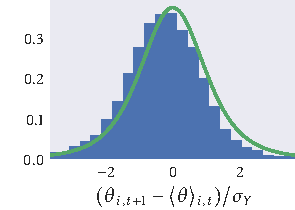
\includegraphics{seq2/top_residuals.pdf}
    \caption{Topological model}
  \end{subfigure}
  \caption{Standardised residuals of models fitted to sequence $2$.}
\end{figure}

\subsubsection{Model rankings}

\subsubsection{Posterior predictive checks}

\subsection{Sequence 3}

\subsubsection{Posterior beliefs}

\begin{figure}[p]
  \captionsetup[subfigure]{aboveskip=0pt,
                           belowskip=9pt,
                           oneside,
                           margin={0.7cm,0cm}}
  \begin{subfigure}[b]{\textwidth}
    \centering
    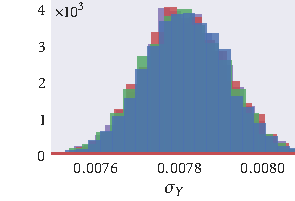
\includegraphics{seq3/null_hist_sigma_Y.pdf}\hspace{0.01\textwidth}
    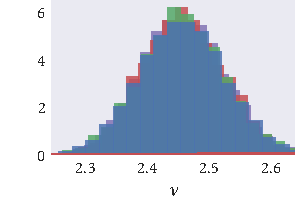
\includegraphics{seq3/null_hist_nu.pdf}
    \caption{Null model}
  \end{subfigure}
  \begin{subfigure}[b]{\textwidth}
    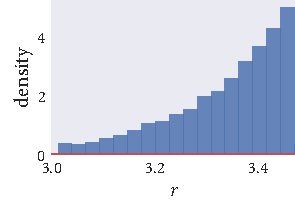
\includegraphics{seq3/r_hist_r.pdf}%
    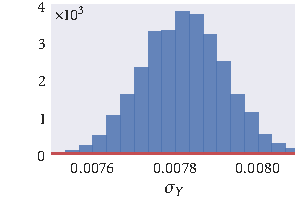
\includegraphics{seq3/r_hist_sigma_Y.pdf}%
    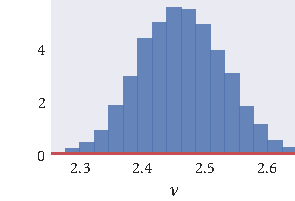
\includegraphics{seq3/r_hist_nu.pdf}
    \caption{Vicsek model}
  \end{subfigure}
  \begin{subfigure}[b]{\textwidth}
    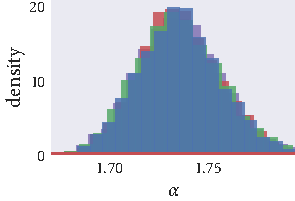
\includegraphics{seq3/power_hist_alpha.pdf}%
    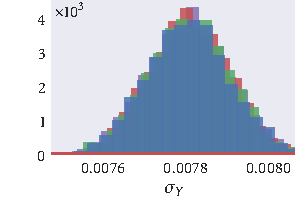
\includegraphics{seq3/power_hist_sigma_Y.pdf}%
    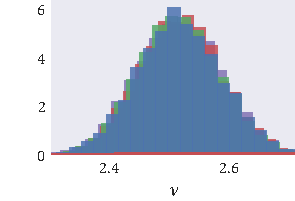
\includegraphics{seq3/power_hist_nu.pdf}
    \caption{Power-law weighted model}
  \end{subfigure}
  \begin{subfigure}[b]{\textwidth}
    \includegraphics{seq3/gauss_hist_sigma_X.pdf}%
    \includegraphics{seq3/gauss_hist_sigma_Y.pdf}%
    \includegraphics{seq3/gauss_hist_nu.pdf}
    \caption{Gaussian weighted model}
  \end{subfigure}
  \begin{subfigure}[b]{\textwidth}
    \includegraphics{seq3/top_hist_k.pdf}%
    \includegraphics{seq3/top_hist_sigma_Y.pdf}%
    \includegraphics{seq3/top_hist_nu.pdf}%
    \caption{Topological model}
  \end{subfigure}
  \caption{Posterior beliefs of model fits to sequence $3$.}
\end{figure}

\subsubsection{Standardised residuals}

\begin{figure}
  \captionsetup[subfigure]{aboveskip=2pt,
                           belowskip=9pt,
                           oneside,
                           margin={0.7cm,0cm}}
  \begin{subfigure}[b]{0.33333\textwidth}
    \caption{Null model}
    \includegraphics{seq3/null_residuals.pdf}
  \end{subfigure}\hspace{2pt}
  \begin{subfigure}[b]{0.33333\textwidth}
    \caption{Vicsek model}
    \includegraphics{seq3/r_residuals.pdf}
  \end{subfigure}\vspace{1em}\\
  \begin{subfigure}[b]{0.33333\textwidth}
    \includegraphics{seq3/power_residuals.pdf}
    \caption{Power-law weighted model}
  \end{subfigure}%
  \begin{subfigure}[b]{0.33333\textwidth}
    \includegraphics{seq3/gauss_residuals.pdf}
    \caption{Gaussian weighted model}
  \end{subfigure}%
  \begin{subfigure}[b]{0.33333\textwidth}
    \includegraphics{seq3/top_residuals.pdf}
    \caption{Topological model}
  \end{subfigure}
  \caption{Standardised residuals of models fitted to sequence $3$.}
\end{figure}

\subsubsection{Model rankings}

\subsubsection{Posterior predictive checks}



